\begin{block}{Syntax-Aware Semantic Role Labeling}
\vspace{-.5\baselineskip}
\begin{itemize}
    \item Semantic Role Labeling predicts semantic dependencies
    \item Semantic dependencies correlate with syntactic dependencies
\end{itemize}
\vspace{-.5\baselineskip}
\begin{figure}
    \centering
    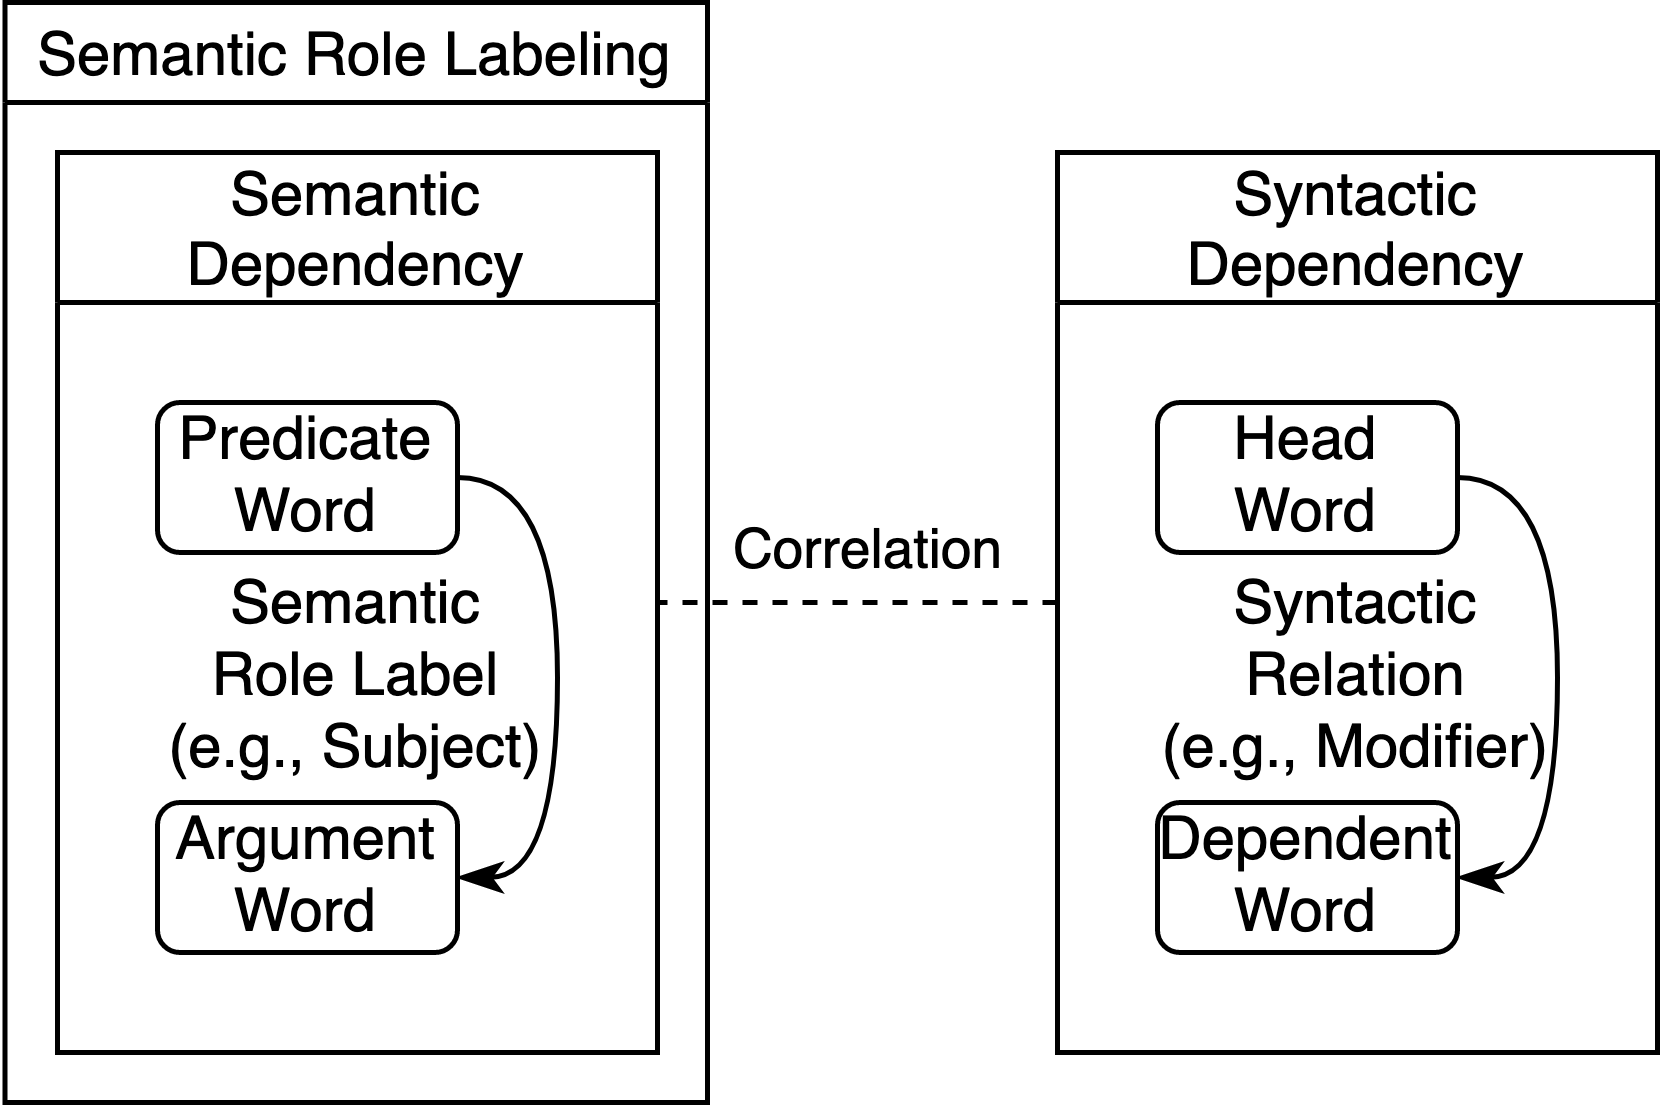
\includegraphics[width=0.8\textwidth]{images/srl-synsem-intro.png}
    \caption{Semantic role labeling and two dependencies}
    \label{fig:my_label}
\end{figure}
\vspace{-.5\baselineskip}
\textbf{Research question: How to \textit{define} and \textit{utilize} the Syntactic-Semantic Dependency Correlation for semantic dependency predictions}
\end{block}


\begin{block}{Concepts}
\vspace{-.5\baselineskip}
\begin{itemize}
    \item Semantic labels denote the relation of semantic dependencies
    \item Hop patterns denote the transition of shortest syntactic dependency paths (SSDP)
\end{itemize}
\vspace{-.5\baselineskip}
\begin{figure}
    \centering
    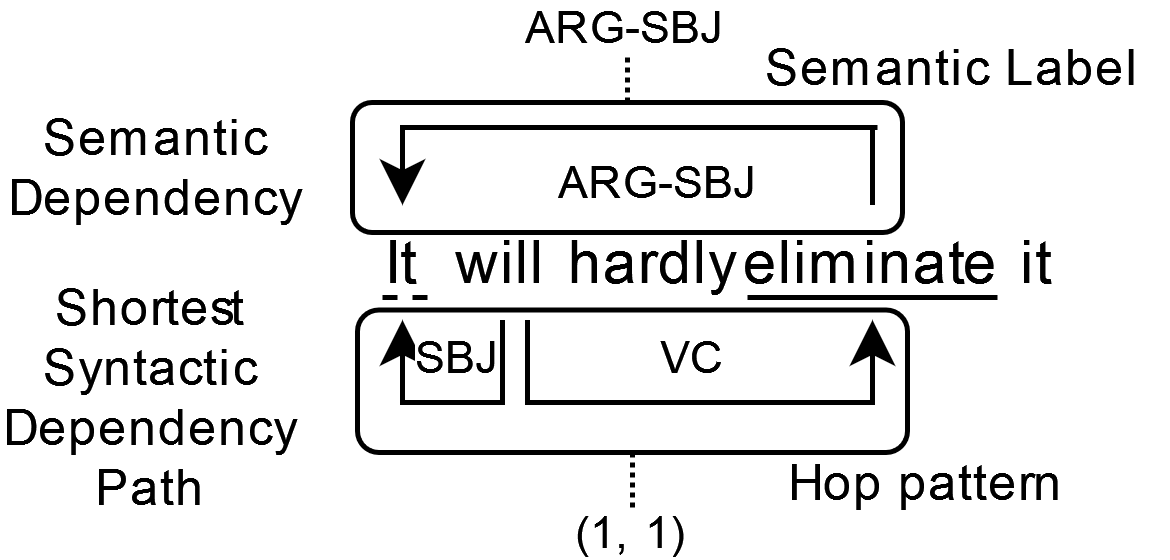
\includegraphics[width=0.8\textwidth]{images/synsem-explanation-3.png}
    \caption{Relevant concepts. The solid underline highlights the \underline{predicate} word and the dashed underline highlights the \dashuline{argument} word}
    \label{fig:my_label}
\end{figure}
\end{block}


% \begin{block}{Motivation}
% We study the syntactic-semantic dependency correlation through the mutual information gain of SSDP hop patterns.
% % \setlist{nolistsep}
% \begin{itemize}
%     % \item Syntactic dependencies: Head$\rightarrow$Dependent relations.
%     % \item Semantic dependencies: Predicate$\rightarrow$Argument relations. We denote the relation type as semantic labels.
%     \vspace{-0.8cm}
%     \item Semantic label: relation type (e.g., A0) of semantic dependencies
%     \item SSDP: Shortest Syntactic Dependency Path connecting predicate-argument pairs
%     \item Hop pattern: the transition pattern of SSDP
% \end{itemize}
% \begin{figure}
%     \centering
%     \captionsetup{justification=centering}
%     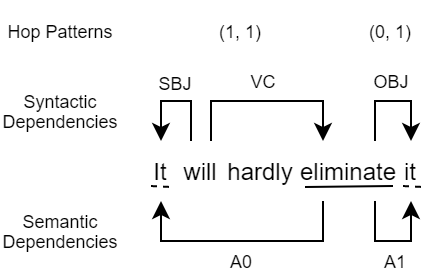
\includegraphics[width=0.7\textwidth]{images/syn-sem-dep-example.png}
%     \caption{Example semantic dependencies, SSDP of the semantic dependencies, and hop patterns. Solid lines underline predicates and dash lines underline arguments.}
%     \label{fig:syn-sem example}
% \end{figure}
% % Hop patterns distinguish the two semantic dependencies with the same predicate-argument pair.\\
% % \vspace{0.5cm}
% % \textbf{Hypothesis: Different hop patterns have unique distributions of semantic labels.}
% Intuitions:
% \begin{itemize}
% \vspace{-1cm}
%     \item Semantic dependencies are modeled as a distribution of the predicate and the argument \cite{dozat-manning-2018-simpler, strubell-etal-2018-linguistically, he-etal-2018-syntax}
%     \item Semantic parsers are vulnerable to semantic dependencies (Figure \ref{fig:syn-sem example}) that have different semantic labels but share the same predicate and argument
%     \item Hop patterns can distinguish between the two semantic dependencies
% \end{itemize}

% \textbf{Hypothesis: Different hop patterns have unique distributions of semantic labels}


% \end{block}